\documentclass{article}

% if you need to pass options to natbib, use, e.g.:
%     \PassOptionsToPackage{numbers, compress}{natbib}
% before loading neurips_2021

% ready for submission
\usepackage[final]{neurips_2021}

% to compile a preprint version, e.g., for submission to arXiv, add add the
% [preprint] option:
%     \usepackage[preprint]{neurips_2021}

% to compile a camera-ready version, add the [final] option, e.g.:
%     \usepackage[final]{neurips_2021}

% to avoid loading the natbib package, add option nonatbib:
%    \usepackage[nonatbib]{neurips_2021}

\usepackage[utf8]{inputenc} % allow utf-8 input
\usepackage[T1]{fontenc}    % use 8-bit T1 fonts
\usepackage{hyperref}       % hyperlinks
\usepackage{url}            % simple URL typesetting
\usepackage{booktabs}       % professional-quality tables
\usepackage{amsfonts}       % blackboard math symbols
\usepackage{nicefrac}       % compact symbols for 1/2, etc.
\usepackage{microtype}      % microtypography
\usepackage{xcolor}         % colors
\usepackage{amsmath}
\usepackage{verbatim}
\usepackage[mathscr]{euscript}
\usepackage{graphicx}
\title{Machine Learning, 2024 Spring\\Assignment 5}
% The \author macro works with any number of authors. There are two commands
% used to separate the names and addresses of multiple authors: \And and \AND.
%
% Using \And between authors leaves it to LaTeX to determine where to break the
% lines. Using \AND forces a line break at that point. So, if LaTeX puts 3 of 4
% authors names on the first line, and the last on the second line, try using
% \AND instead of \And before the third author name.



\begin{document}
\author{
    Name: \textbf{Zhou Shouchen} \\
	Student ID: 2021533042
}
\maketitle

\begin{abstract}

\end{abstract}
\newpage

\textcolor{blue}{Problem 1}

Which of the following are possible growth functions $m_{\mathcal{H}}(N)$ for some hypothesis set:
$$
1+N ; 1+N+\dfrac{N(N-1)}{2} ; 2^N ; 2^{\lfloor\sqrt{N}\rfloor} ; 2^{\lfloor \frac{N}{2} \rfloor} ; 1+N+\dfrac{N(N-1)(N-2)}{6}
$$

\textcolor{blue}{Solution}\\
\begin{itemize}
    \item[1. ] $1+N$:\\
    Since $1+1=2^1$, and $1+2<2^2$, so $k=2$ is the breakpoint.
    $$\sum_{i=0}^{k-1} \binom{N}{i} = \sum_{i=0}^{1} \binom{N}{i} = 1+N$$
    Since $$m_{\mathcal{H}}(N)=1+N\leq \sum_{i=0}^{k-1} \binom{N}{i}$$
    So $m_{\mathcal{H}}(N)=1+N$ is a possible growth function.
    
    \item[2. ]  $1+N+\dfrac{N(N-1)}{2}$:\\
    Since $1+2+\dfrac{2*1}{2}=2^2$, and $1+3+\dfrac{3*2}{2}<2^3$, so $k=3$ is the breakpoint.
    $$\sum_{i=0}^{k-1} \binom{N}{i} = \sum_{i=0}^{2} \binom{N}{i} = 1+N+\dfrac{N(N-1)}{2}$$
    So $$m_{\mathcal{H}}(N)=1+N+\dfrac{N(N-1)}{2}\leq \sum_{i=0}^{k-1} \binom{N}{i}$$
    So $m_{\mathcal{H}}(N)=1+N+\dfrac{N(N-1)}{2}$ is a possible growth function.
    
    \item[3. ] $2^N$:\\
    $\forall k=1,2,\cdots,N$, we have
    $$m_{\mathcal{H}}(N)=2^N$$
    So the breakpoint is $k=\infty$.
    $$\sum_{i=0}^{k-1} \binom{N}{i} = 2^N$$
    So $$m_{\mathcal{H}}(N)=2^N\leq \sum_{i=0}^{k-1} \binom{N}{i}$$
    So $m_{\mathcal{H}}(N)=2^N$ is a possible growth function.
    
    \item[4.] $2^{\lfloor\sqrt{N}\rfloor}$:\\
    Since $2^{\lfloor\sqrt{1}\rfloor}=2^1$ and $2^{\lfloor\sqrt{2}\rfloor}<2^2$, so $k=2$ is the breakpoint.
    $$\sum_{i=0}^{k-1} \binom{N}{i} = \sum_{i=0}^{1} \binom{N}{i} = 1+N$$
    But $m_{\mathcal{H}}(N)=2^{\lfloor\sqrt{N}\rfloor}$ is close to a exponential function, and the $1+N$ is polynormial function, so it must has a $N$, such as $N=25$:
    $$m_{\mathcal{H}}(N)=32>1+N=26$$
    So $m_{\mathcal{H}}(N)=2^{\lfloor\sqrt{N}\rfloor}$ is not a possible growth function.

    \item[5.] $2^{\lfloor \frac{N}{2} \rfloor}$:\\
    Since $2^{\lfloor \frac{0}{2}\rfloor}=2^0$ and $2^{\lfloor \frac{1}{2}\rfloor}=1<2^1$, so $k=1$ is the breakpoint.
    $$\sum_{i=0}^{k-1} \binom{N}{i} = \sum_{i=0}^{0} \binom{N}{i} = 1$$
    But $m_{\mathcal{H}}(N)=2^{\lfloor\frac{N}{2}\rfloor}$ is an increasing function, and the $1$ is a constant function, so $\forall N\geq 2$
    $$m_{\mathcal{H}}(N)=2^{\lfloor \frac{N}{2}\rfloor}>1$$
    So $m_{\mathcal{H}}(N)=2^{\lfloor \frac{N}{2}\rfloor}$ is not a possible growth function.
    
    \item[6.] $1+N+\dfrac{N(N-1)(N-2)}{6}$:\\
    Since $1+1+\dfrac{1(1-1)(1-2)}{6}=2^1$ and $1+2+\dfrac{2(2-1)(2-2)}{6}=3<2^2$, so $k=2$ is the breakpoint.
    $$\sum_{i=0}^{k-1} \binom{N}{i} = \sum_{i=2}^{0} \binom{N}{i} = 1+N$$
    But when $\dfrac{N(N-1)(N-2)}{6}\neq 0$, i.e. $N\geq 3$, we have
    $$m_{\mathcal{H}}(N)=1+N+\dfrac{N(N-1)(N-2)}{6}>1+N$$
    So $m_{\mathcal{H}}(N)=1+N+\dfrac{N(N-1)(N-2)}{6}$ is not a possible growth function.
    
\end{itemize}
So above all, the possible growth functions $m_{\mathcal{H}}(N)$ are 
$$1+N ; 1+N+\dfrac{N(N-1)}{2}; 2^N $$
And the followings are not possible growth functions.
$$ 2^{\lfloor\sqrt{N}\rfloor} ; 2^{\lfloor \frac{N}{2} \rfloor}; 1+N+\dfrac{N(N-1)(N-2)}{6} $$

\newpage
\textcolor{blue}{Problem 2}

For an $\mathcal{H}$ with $d_{\mathrm{vc}}=10$, what sample size do you need (as prescribed by the generalization bound) to have a $95 \%$ confidence that your generalization error is at most 0.05 ?

\textcolor{blue}{Solution}\\








\newpage
\textcolor{blue}{Problem 3}
According to the iterative format provided as follow:
\begin{itemize}
    \item Use the SUV dataset to implement (using Python or MATLAB) the Gradient Descent method to find the optimal model for logistic regression.
    \item What is your test error? What are the sizes of the training set and test set, respectively?
    \item What is your learning rate? How was it chosen? How many steps were iterated in total?
    \item Present the results of the last 10 steps produced by your algorithm, including the loss, learning rate, the L2 norm of the gradient, and the number of function evaluations and gradient evaluations.
\end{itemize}
\begin{figure}[htbp]
\centerline{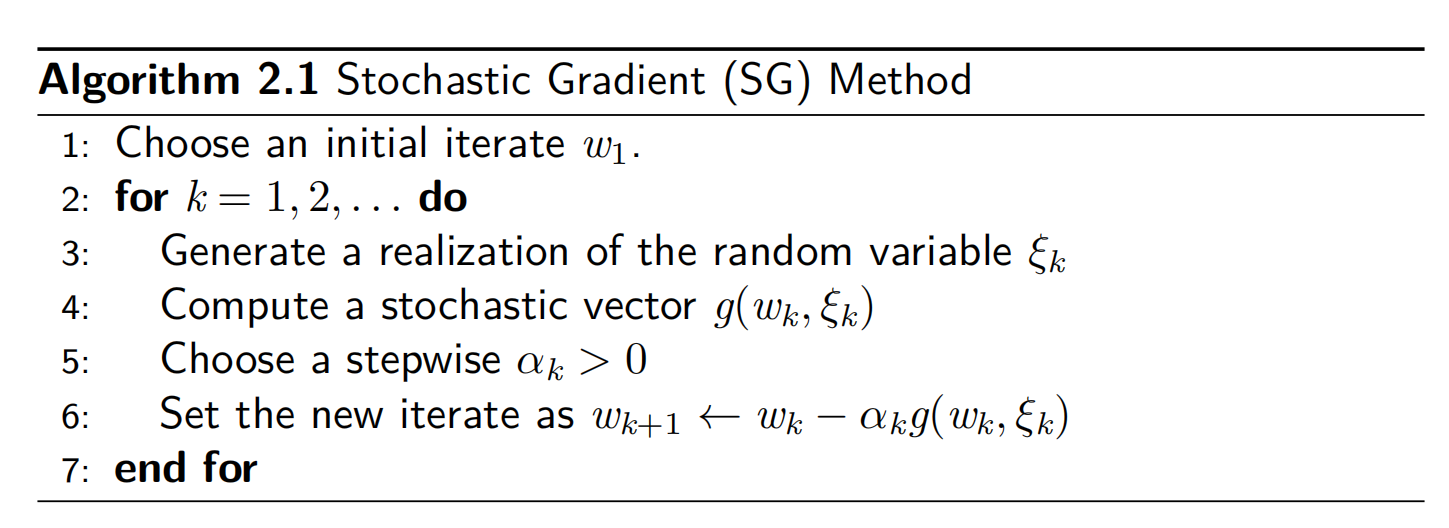
\includegraphics[width=\textwidth]{../image/alg.png}}
\href
  {https://www.cs.toronto.edu/~mhsadi/code-repository/MachineLearningNotebooks/3-SUVDataset.html}
  {Dataset reference and description}
  \\
\href
{https://www.kaggle.com/datasets/iamaniket/suv-data?resource=download}
  {Dataset and download}

\end{figure}

\textcolor{blue}{Solution}

0. Data preperation\\
After checking the SUV dataset, we could find that each buyer's information has a unique `User ID', so we can just drop the `User ID' column.\\
To use the `Gender' information, we map `Male' into $1$, and `Female' into $0$.\\
If we use exponential function during the logistic regression, it may have too big values with large `Age' and `EstimatedSalary', so we can seperate the `Age' and `EstimatedSalary' into different intervals.
And use an one-hot vector to represent the which range the `Age' and `EstimatedSalary' belongs to. And the modified encoding for `Age' and `Estimated salary' are as followed in Figure \ref{fig:age} and Figure \ref{fig:salary}.
The catagoies of `Age' and `EstimatedSalary' are chosen by the distribution graph of the original data, and each catagory is represented by a one-hot vector.\\

\begin{figure}[htbp]
  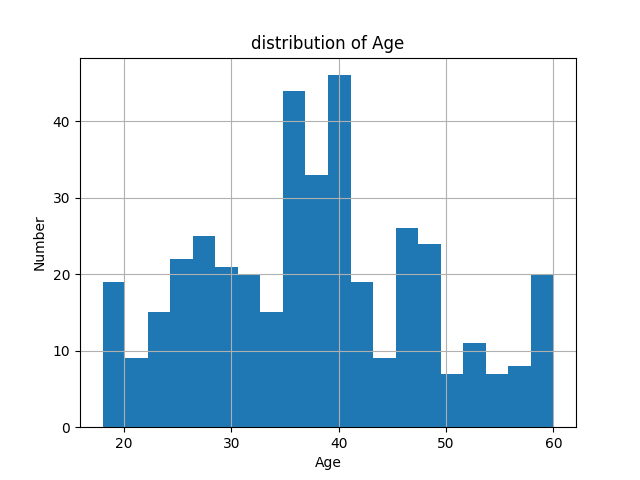
\includegraphics[width=0.5\textwidth]{../image/age_distribution.png}
  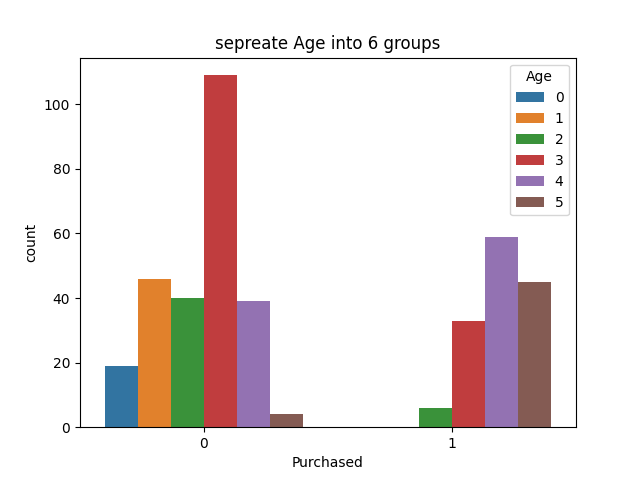
\includegraphics[width=0.5\textwidth]{../image/seperated_age.png}
  \caption{Analysis of Age}  
\label{fig:age}
\end{figure}

\begin{figure}[htbp]
  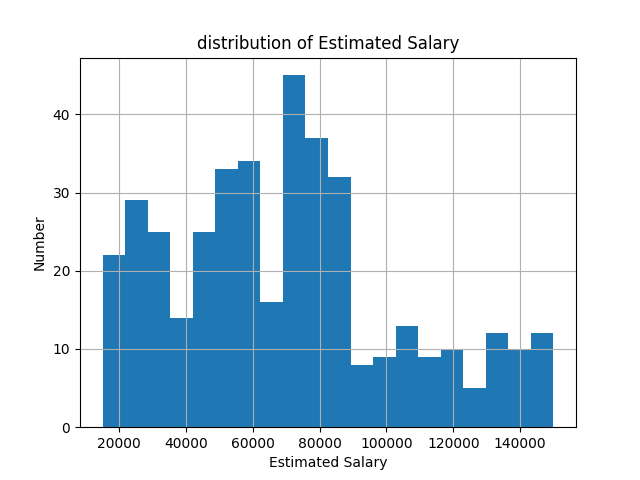
\includegraphics[width=0.5\textwidth]{../image/salary_distribution.png}
  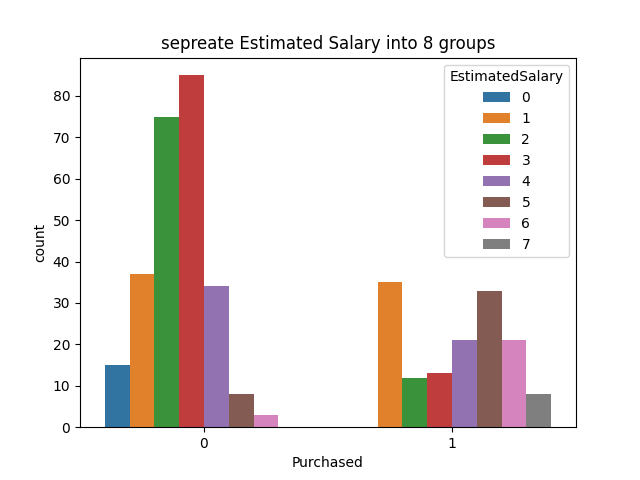
\includegraphics[width=0.5\textwidth]{../image/seperated_salary.png}
  \caption{Analysis of Estimated Salary}  
\label{fig:salary}
\end{figure}

To suit better for logistic regression, the `Purchased' column is also modified into `$-1$' for unpurchased and `$1$' for purchased.\\
At last, a bias term `$1$ is add for each input fetures. 
And before sending the data into the logistic regression, the input features are normalized.\\

Then the `Gender', `Age', `EstimatedSalary' can be used as the input features, and the `Purchased' can be used as the output label.\\
So this is a binary classification problem.\\
And we can use the logistic regression to solve this problem.\\

1. Since we are applying the logistic regression, so the testing error is:
$$E(\mathbf{w}) = \dfrac{1}{N}\sum_{i=1}^{N}\log (1+e^{-y_n\mathbf{w}^T\mathbf{x}_n})$$
which have been proved in Problem 1. And $N$ is the size of the testing set's size. $y_n$ are the labels of
testing set, $\mathbf{x}_n$ are the input data for the testing set.\\
The variation curve for the testing error is shown in Figure \ref{fig:testing}.\\

And the size of training set is $70$ persent, which is totally $280$ samples. And the testing set is $30$ persent, which is totally $120$ samples.\\
And before seperating the data, we random shuffled the total $400$ data with a fixed seed in order to make sure the randomness, but could be stable reproduction.\\

2. We have known that the gradient of logistic regression from Problem 1 is:
$$\nabla E_{\text {in }}(\mathbf{w}) = \dfrac{1}{N}\sum_{i=1}^{N}-y_n\mathbf{x}_n\theta(-y_n\mathbf{w}^T\mathbf{x}_n)$$
$\nabla E_{\text {in }}(\mathbf{w}),y_n,\mathbf{x}_n$ are set for the training set.\\
To set the learning rate getting smaller as the training iterations go on, we can set the learning rate as:
$$\eta_t = \eta\cdot \|\nabla E_{\text{in}}(\mathbf{w})\|$$
where $\eta=0.2$ is the initial learning rate, and $\|\nabla E_{\text{in}}(\mathbf{w})\|$ is the norm of the gradient.\\
And the total iterated steps is set to be $5000$ iterataions.\\ 

3. The results of the last 10 steps are shown in Figure \ref{fig:info}.\\
We could see that the training loss, the $L_2$ norm of the gradient $\|\nabla E_{\text{in}}(\mathbf{w})\|$ are dropping, but quite slow, which is close to get converage.\\
And the number of the gradient evaluations is once per iterataion, used for updating the $\mathbf{w}$.\\
And the number of the gradient evaluations is twice per iterataion, used for calculating the loss for both training set and the testing set.\\

\begin{figure}[htbp]
  \centerline{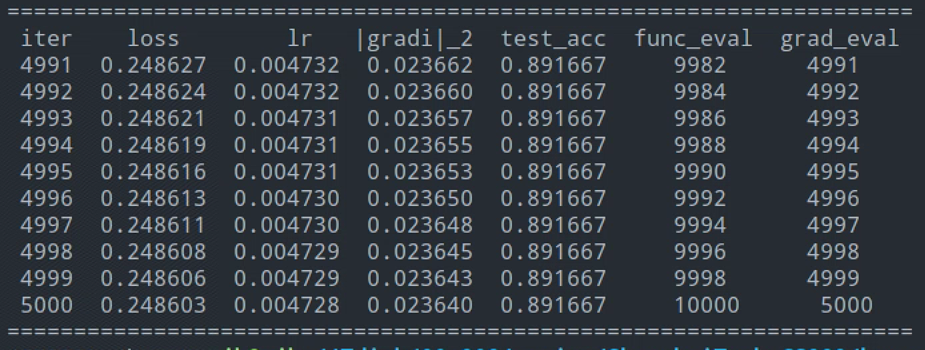
\includegraphics[width=\textwidth]{../image/info.png}}
  \caption{The last 10 steps' output} 
  \label{fig:info} 
\end{figure}

4. Analysis:\\
Figure \ref{fig:testing} are the testing accuracy and testing loss. From the 
testing loss, we could find that the model somehow overfitted on the training data, as the 
testing loss gradually becomes higher as the iterataions grow. But the testing accuracy was not effected so much,
it might because the dataset is small, and the data distribution are regular, so overfitting on the training set did not make testing accuracy got worse.\\

Figure \ref{fig:training} are the gradient's $L_2$ norm $\|\nabla E_{\text{in}}(\mathbf{w})\|$, the learning rate $\eta_t = \eta\cdot \|\nabla E_{\text{in}}(\mathbf{w})\|$, and the training loss.\\
The learning rate is obviously to have the same trend with the $\|\nabla E_{\text{in}}(\mathbf{w})\|$ as they have the proportional relationship. The training loss also has the 
quite same trend with them. Decreasing rapidly at first, and getting much slower as getting converage.\\

5. The code and the method to run the code are all in the folder `code'.

\begin{figure}[htbp]
  \centerline{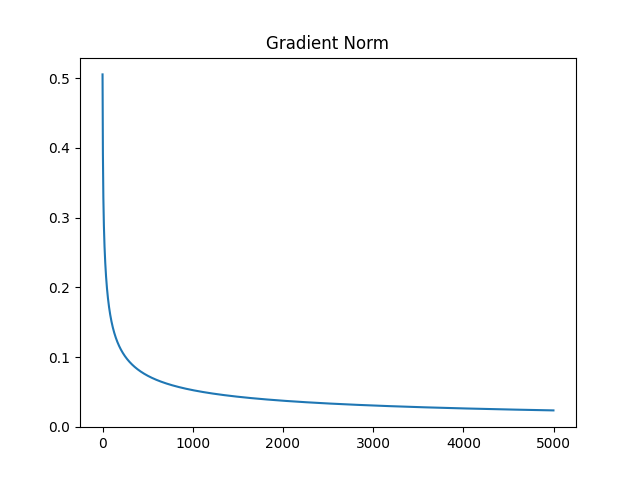
\includegraphics[width=0.7\textwidth]{../image/grad_norm.png}}
  \centerline{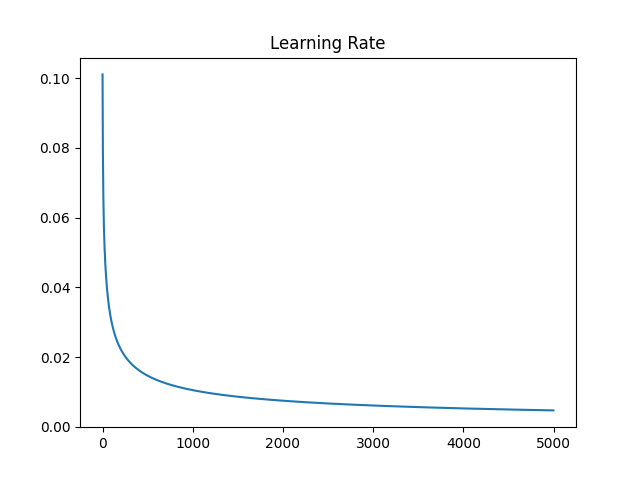
\includegraphics[width=0.7\textwidth]{../image/learning_rate.png}}
  \centerline{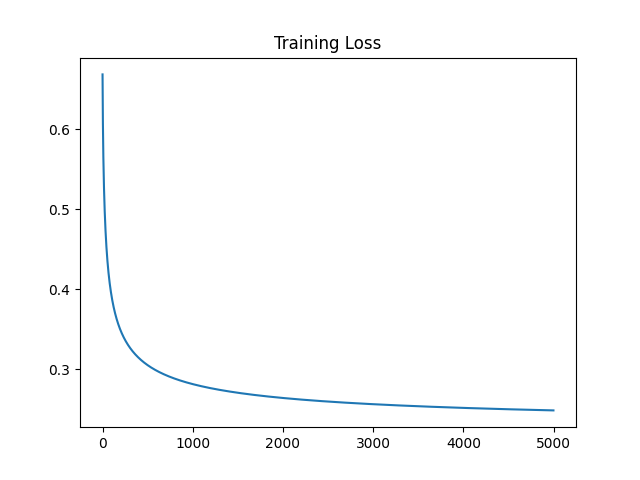
\includegraphics[width=0.7\textwidth]{../image/training_loss.png}}
  \caption{The training information}
  \label{fig:training}
\end{figure}

\begin{figure}[htbp]
  \centerline{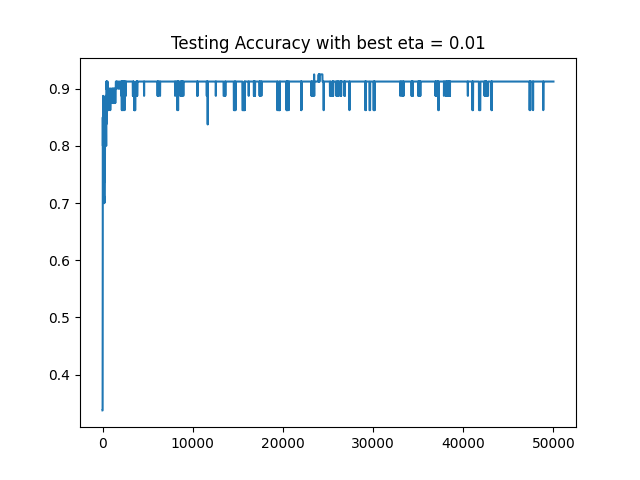
\includegraphics[width=\textwidth]{../image/testing_acc.png}}
  \centerline{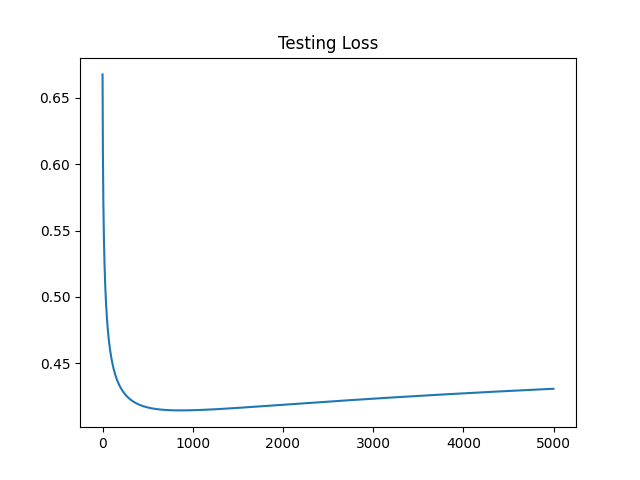
\includegraphics[width=\textwidth]{../image/testing_loss.png}}
  \caption{The testing information}
  \label{fig:testing}
\end{figure}
\textcolor{blue}{Problem 4}

Let $\mathcal{H}_1, \mathcal{H}_2, \ldots, \mathcal{H}_K$ be $K$ hypothesis sets with finite VC dimension $d_{\text {vc }}$. Let $\mathcal{H}=\mathcal{H}_1 \cup \mathcal{H}_2 \cup \ldots \cup \mathcal{H}_K$ be the union of these models. Show that $d_{\mathrm{vc}}(\mathcal{H})<K\left(d_{\mathrm{vc}}+1\right)$.

\textcolor{blue}{Solution}\\













\newpage
\textcolor{blue}{Problem 5}

In this part, you need to complete some mathematical proofs about VC dimension. Suppose the hypothesis set
$$
\mathcal{H}=\{f(x, \alpha)=\operatorname{sign}(\sin (\alpha x)) \mid, \alpha \in \mathbb{R}\}
$$
where $x$ and $f$ are feature and label, respectively.
\begin{itemize}
    \item Show that $\mathcal{H}$ cannot shatter the points $x_1=1, x_2=2, x_3=3, x_4=4$.
\end{itemize}
(Key: Mathematically, you need to show that there exists $y_1, y_2, y_3, y_4$, for any $\alpha \in \mathbb{R}, f\left(x_i\right) \neq$ $y_i, i=1,2,3,4$, for example, $+1,+1,-1,+1$ )
\begin{itemize}
\item Show that the VC dimension of $\mathcal{H}$ is $\infty$. (Note the difference between it and the first question)
\end{itemize}
(Key: Mathematically, you have to prove that for any label sets $y_1, \cdots, y_m, m \in \mathbb{N}$, there exists $\alpha \in \mathbb{R}$ and $x_i, i=1,2, \cdots, m$ such that $f(x ; \alpha)$ can generate this set of labels. Consider the points $\left.x_i=10^{-i} \ldots\right)$

\textcolor{blue}{Solution}\\
(1) For the case $x_1=1, x_2=2, x_3=3, x_4=4$ with label $y_1=+1$, $y_2=+1$, $y_3=-1$, $y_4=+1$,
we can prove that $\forall\alpha\in\mathbb{R},\exists i\in\{1,2,3,4\},f(x_i)\neq y_i$.
\begin{itemize}
    \item 1. For $x_1=1$\\
    Since $y_1=+1$, we have $f(x_1)=\text{sign}(\sin\alpha)=+1\Rightarrow \sin\alpha>0$\\
    i.e. we have $\sin\alpha>0$.

    \item 2. For $x_2=2$\\
    Since $y_2=+1$, we have $f(x_2)=\text{sign}(\sin 2\alpha)=+1\Rightarrow \sin 2\alpha>0$\\
    i.e. we have $\sin 2\alpha=2\sin\alpha\cos\alpha>0$.\\
    From 1. we have known that $\sin\alpha>0$, so we must have $\cos\alpha>0$.\\
    i.e. we have $\cos\alpha>0$ and $\sin 2\alpha>0$.
    
    \item For $x_3=3$\\ 
    Since $y_3=-1$, we have $f(x_3)=\text{sign}(\sin 3\alpha)=-1\Rightarrow \sin 3\alpha<0$\\
    i.e. we have $\sin 3\alpha=\sin\alpha\cos 2\alpha+\sin 2\alpha\cos\alpha<0$.\\
    From 1. we have $\sin\alpha>0$, and from 2. we have $\cos\alpha>0$, $\sin 2\alpha>0$,\\
    so we must have $\cos 2\alpha<0$.\\
    i.e. we have $\cos 2\alpha<0$.

    \item For $x_4=4$\\
    Since $y_4=+1$, we have $f(x_4)=\text{sign}(\sin 4\alpha)=+1\Rightarrow \sin 4\alpha>0$\\
    i.e. we have $\sin(4\alpha)=2\sin(2\alpha)\cos(2\alpha)>0$\\
    But from 2. we have $\sin 2\alpha>0$, from 3. we have $\cos 2\alpha<0$,\\
    so we must have $\sin(4\alpha)<0$, which is a contradiction.
\end{itemize}

So we have prove that for $y_1=+1$, $y_2=+1$, $y_3=-1$, $y_4=+1$, \\$\forall\alpha\in\mathbb{R}$, if $\forall i\in\{1,2,3\},f(x_i)= y_i$, then $f(x_4)\neq y_4$.\\
So above all, $\mathcal{H}$ cannot shatter the points $x_1=1, x_2=2, x_3=3, x_4=4, \ \forall \alpha\in\mathbb{R}$.\\

(2) We can construct that:\\
Let $\alpha=1$, $x_i=\pi-\dfrac{\pi}{2}\cdot y_i+2\pi i, i=1,2,\cdots, m$\\
\begin{itemize}
    \item For $y_i=+1$, we have
    $$f(x_i)=\text{sign}(\sin(\pi-\dfrac{\pi}{2}\cdot y_i+2\pi i))=\text{sign}(\sin(\dfrac{\pi}{2}+2\pi i))=+1$$
    \item For $y_i=-1$, we have 
    $$f(x_i)=\text{sign}(\sin(\pi-\dfrac{\pi}{2}\cdot y_i+2\pi i))=\text{sign}(\sin(\dfrac{3\pi}{2}+2\pi i))=-1$$
\end{itemize}

So above all, we have proved that for any label sets $y_1, \cdots, y_m, m \in \mathbb{N}$, \\there exists $\alpha \in \mathbb{R}$ and $x_i, i=1,2, \cdots, m$ such that $f(x ; \alpha)$ can generate this set of labels.\\
i.e. the VC dimension of $\mathcal{H}$ is $\infty$.


\end{document}